\chapter{Исследовательская часть}

\section{Технические характеристики}

Технические характеристики устройства, на котором выполнялись замеры по времени, представлены далее.

\begin{itemize}
	\item Процессор: Intel(R) Core(TM) i5-10300H CPU 2.50 ГГц \cite{intel}.
	\item Оперативная память: 16 ГБайт.
	\item Операционная система: Windows 10 Pro 64-разрядная система версии 21H2 \cite{windows}.
\end{itemize}

При замерах времени ноутбук был включен в сеть электропитания и был нагружен только системными приложениями.

\section{Демонстрация работы программы}

%Тут абзац со ссылкой на рисунок и описанием того, что на нём представлено/происходит
На рисунке \ref{img:demonstration} представлена демонстрация работы разработанного программного обеспечения, а именно показаны результаты вычислений реализаций алгоритмов поиска расстояний Левенштейна и Дамерау-Левенштейна на примере двух строк <<друзья>> и <<рдузия>>. При этом выводятся матрицы для алгоритмов, использующих матрицы для промежуточных результатов.  
\clearpage
\begin{figure}[h]
	\centering
	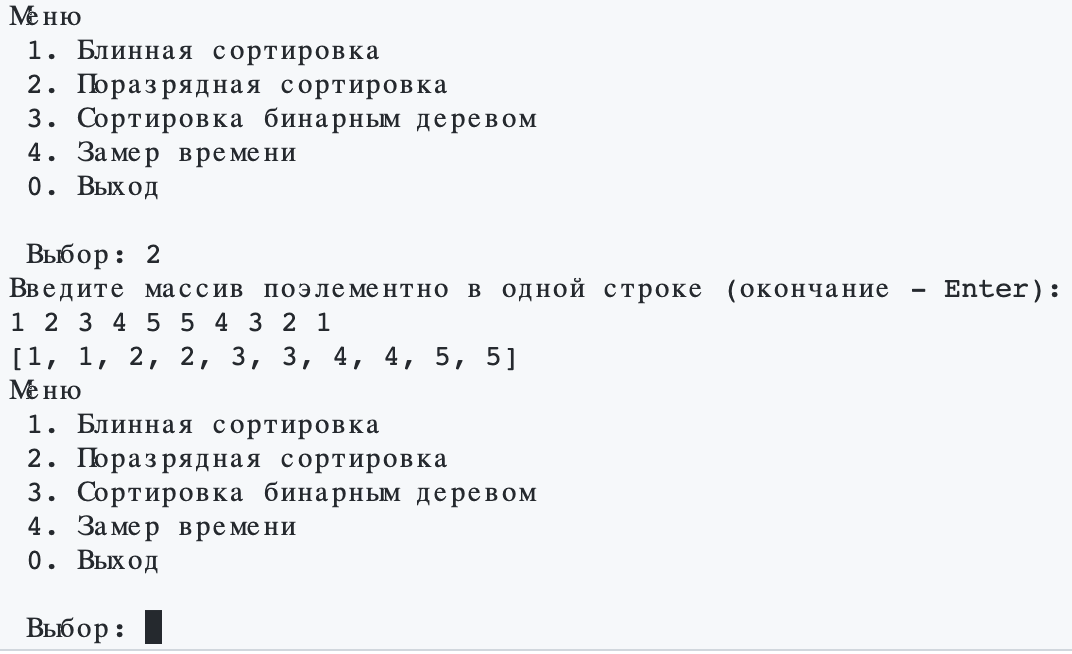
\includegraphics[height=0.7\textheight]{img/example.png}
	\caption{Демонстрация работы программы при поиске расстояний Левенштейна и Дамерау-Левенштейна}
	\label{img:demonstration}
\end{figure}

\clearpage

\section{Временные характеристики}

Результаты эксперимента замеров по времени приведены в таблице \ref{tbl:time}, в которой есть поля, обозначенные <<\-->>. Это обусловлено тем, что для рекурсивной реализации алгоритмов достаточно приведенных замеров для построения графика. По полученным замерам по времени для рекурсивной реализации понятно, что проведения замеров на длин строк больше 15 будет достаточно долгим, поэтому нет смысла проводить замеры по времени рекурсивных реализаций алгоритмов поиска расстояния.

Замеры проводились на одинаковых длин строк от 1 до 200 с различным шагом.
% по точке выравнивание
\begin{table}[ht]
	\small
	\begin{center}
		\begin{threeparttable}
		\caption{Замер по времени для строк, размер которых от 1 до 200}
		\label{tbl:time}
		\begin{tabular}{|c|c|c|c|c|}
			\hline
			& \multicolumn{4}{c|}{\bfseries Время, нс} \\ \cline{2-5}
			& \multicolumn{1}{c|}{\bfseries Левенштейн}
			& \multicolumn{3}{c|}{\bfseries Дамерау-Левенштейн} \\ \cline{2-5}
			\bfseries Длина (символ) & \bfseries Итеративный & \bfseries Итеративный & \multicolumn{2}{c|}{\bfseries Рекурсивный} \\ \cline{4-5}
			& & & \bfseries Без кеша & \bfseries С кешом
			\csvreader{csv/time.csv}{}
			{\\\hline \csvcoli & \csvcolii & \csvcoliii & \csvcoliv & \csvcolv} \\
			\hline
		\end{tabular}			
		\end{threeparttable}
	\end{center}
\end{table}

Отдельно сравнивается итеративные алгоритмы поиска расстояний Левенштейна и Дамерау--Левенштейна. Сравнение будет производится на основе данных, представленных в таблице \ref{tbl:time}. Результат можно рассмотреть на рисунке \ref{plt:time_01}.

При длинах строк менее 30 символов разница по времени между итеративными реализациями незначительна, однако при увеличении длины строки алгоритм поиска расстояния Левенштейна оказывается быстрее вплоть до полутора раз (при длинах строк равных 200). 
Это обосновывается тем, что у алгоритма поиска расстояния Дамерау-Левенштейна задействуется дополнительная операция, которая замедляет алгоритм.

\begin{figure}[h]
	\centering
	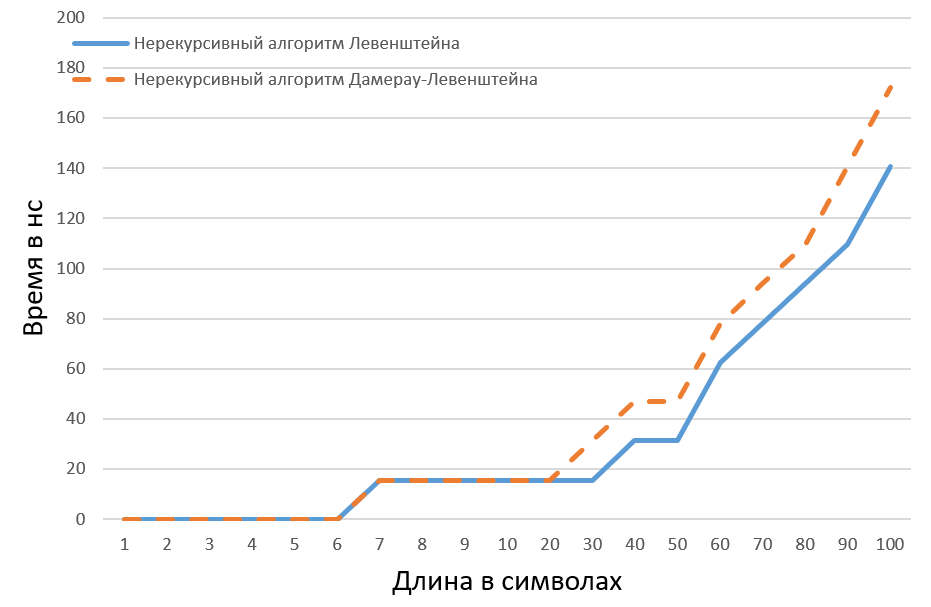
\includegraphics[height=0.3\textheight]{img/diag_01.png}
	\caption{Сравнение по времени нерекурсивных реализаций алгоритмов поиска расстояний Левенштейна и Дамерау-Левенштейна}
	\label{plt:time_01}
\end{figure}

Также сравним рекурсивную и итеративную реализации алгоритма поиска расстояния Дамерау-Левенштейна. Данные представлены в таблице \ref{tbl:time} и отображены на рисунке \ref{plt:time_02}.

\begin{figure}[h]
	\centering
	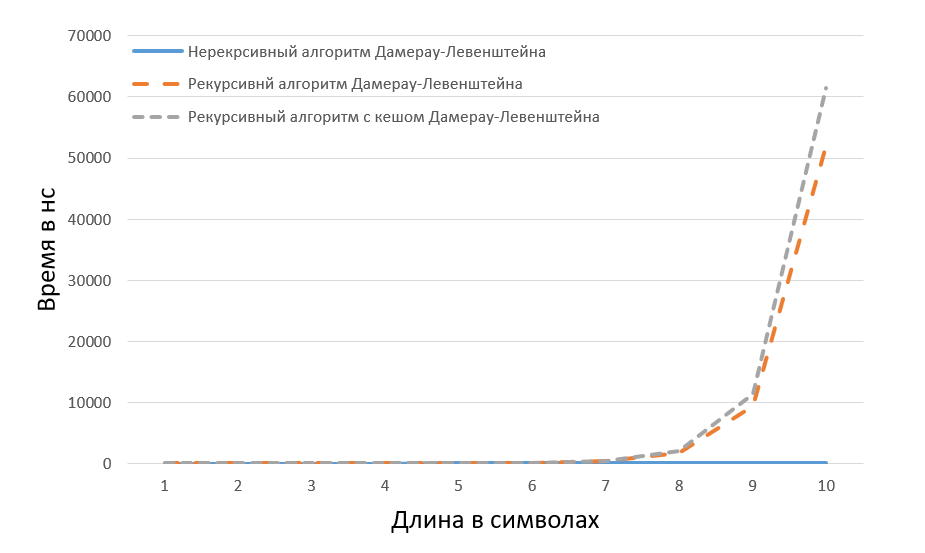
\includegraphics[height=0.3\textheight]{img/diag_02.png}
	\caption{Сравнение по времени алгоритмов поиска расстояния Дамерау-Левенштейна}
	\label{plt:time_02}
\end{figure}

На рисунке \ref{plt:time_02} продемонстрировано, что рекурсивный алгоритм становится менее эффективным по времени (вплоть до 21 раз при длине строк равной 7 элементов), чем итеративный.

Кроме того, согласно данным, приведенным в таблице \ref{tbl:time}, рекурсивные алгоритмы при длинах строк более 10 элементов не пригодны к использованию в силу экспоненциально роста затрат процессорного времени, в то время, как затраты итеративных алгоритмов по времени линейны.

\section{Характеристики по памяти}

Введем следующие обозначения:
\begin{itemize}
	\item$n$ --- длина строки $S_{1}$;
	\item$m$ --- длина строки $S_{2}$;
	\item$size()$ --- функция вычисляющая размер в байтах;
	\item $string$ --- строковый тип;
	\item $int$ --- целочисленный тип;
	\item $size\_t$ --- беззнаковый целочисленный тип.
\end{itemize}

Максимальная глубина стека вызовов при рекурсивной реализации нахождения расстояния Дамерау-Левенштейна равна сумме входящих строк, а на каждый вызов требуется 2 дополнительные переменные, соответственно, максимальный расход памяти равен:
\begin{equation}
	\label{eq:dl_rec_memory}
	(n + m) \cdot (2 \cdot size(string) + 3 \cdot size(int) + 2 \cdot sizeof(size\_t)),
\end{equation}
где:
\begin{itemize}
	\item $2 \cdot size(string)$ --- хранение двух строк;
	\item $2 \cdot size(size\_t)$ --- хранение размеров строк;
	\item $2 \cdot size(int)$ --- дополнительные переменные;
	\item $size(int)$ --- адрес возврата.
\end{itemize}

Для рекурсивного алгоритма c кешированием поиска расстояния Дамерау-Левенштейна будет теоретически схож с расчетом в формуле (\ref{eq:dl_rec_memory}), но также учитывается матрица, соответственно, максимальный расход памяти равен:
\begin{equation}
	\label{eq:dl_hash_memory}
	\begin{aligned}
		(n + m) \cdot (2 \cdot size(string) + 3 \cdot size(int) + 2 \cdot size(size\_t)) + \\
		+ (n + 1) \cdot (m + 1) \cdot size(int)
	\end{aligned}
\end{equation}
Использование памяти при итеративной реализации алгоритма поиска расстояния Левенштейна теоретически равно:
\begin{equation}
	\label{eq:lev_mtr_memory}
	\begin{aligned}
		(n + 1) \cdot (m + 1) \cdot size(int) + 2 \cdot size(string) + 2 \cdot size(size\_t) + \\
		+ size(int **) + (n + 1) \cdot size(int *) + 2 \cdot size(int),
	\end{aligned}
\end{equation}
где 
\begin{itemize}
	\item $2 \cdot size(string)$ --- хранение двух строк;
	\item $2 \cdot size(size\_t)$ --- хранение размеров матрицы;
	\item $(n + 1) \cdot (m + 1) \cdot size(int)$ --- хранение матрицы;
	\item $size(int **) + (n + 1) \cdot size(int *)$ --- указатель на матрицу;
	\item $size(int)$ --- дополнительная переменная для хранения результата;
	\item $size(int)$ --- адрес возврата.
\end{itemize}

Использование памяти при итеративной реализации алгоритма поиска расстояния Дамерау-Левенштейна теоретически равно:
\begin{equation}
	\label{eq:dl_mtr_memory}
	\begin{aligned}
		(n + 1) \cdot (m + 1) \cdot size(int) + 2 \cdot size(string) + 2 \cdot size(size\_t) + \\
		+ size(int **) + (n + 1) \cdot size(int *) + 3 \cdot size(int),
	\end{aligned}
\end{equation}
где 
\begin{itemize}
	\item $2 * size(string)$ --- хранение двух строк;
	\item $2 \cdot size(size\_t)$ --- хранение размеров матрицы;
	\item $(n + 1) \cdot (m + 1) \cdot size(int)$ --- хранение матрицы;
	\item $size(int **) + (n + 1) \cdot size(int *)$ --- указатель на матрицу;
	\item $2 \cdot size(int)$ --- дополнительные переменные;
	\item $size(int)$ --- адрес возврата.
\end{itemize}

По расходу памяти итеративные алгоритмы проигрывают рекурсивным: максимальный размер используемой памяти в итеративном растет как произведение длин строк, в то время как у рекурсивного алгоритма — как сумма длин строк.

По формулам \ref{eq:dl_rec_memory} -- \ref{eq:lev_mtr_memory} затрат по памяти в программе были написаны соответствующие функции для подсчета расходуемой памяти, результаты расчетов, которых представлены в таблице \ref{tbl:memory}, где размеры строк находятся в диапазоне от 10 до 200 с шагом 10.

\clearpage

\begin{table}[ht]
	\small
	\begin{center}
		\begin{threeparttable}
		\caption{Замер памяти для строк, размером от 10 до 200}
		\label{tbl:memory}
		\begin{tabular}{|c|c|c|c|c|}
			\hline
			& \multicolumn{4}{c|}{\bfseries Размер в байтах} \\ \cline{2-5}
			& \multicolumn{1}{c|}{\bfseries Левенштейн}
			& \multicolumn{3}{c|}{\bfseries Дамерау-Левенштейн} \\ \cline{2-5}
			\bfseries Длина (символ) & \bfseries Итеративный & \bfseries Итеративный & \multicolumn{2}{c|}{\bfseries Рекурсивный} \\ \cline{4-5}
			& & & \bfseries Без кеша & \bfseries С кешом
			\csvreader{csv/memory.csv}{}
			{\\\hline \csvcoli & \csvcolii & \csvcoliii & \csvcoliv & \csvcolv} \\
			\hline
		\end{tabular}	
		\end{threeparttable}
	\end{center}
\end{table}

Из данных, приведенных в таблице \ref{tbl:memory}, понятно, что рекурсивные алгоритмы являются более эффективными по памяти, так как используется только память под локальные переменные, передаваемые аргументы и возвращаемое значение, в то время как итеративные алгоритмы затрачивают память линейно пропорционально длинам обрабатываемых строк.

\begin{figure}[h]
	\centering
	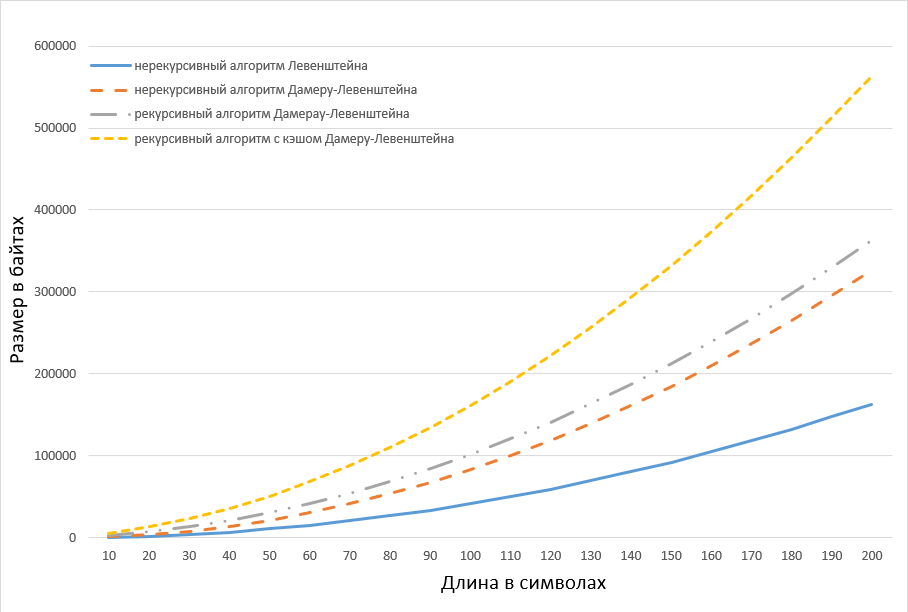
\includegraphics[height=0.3\textheight]{img/diag_03.png}
	\caption{Сравнение по памяти алгоритмов поиска расстояния Левенштейна и Дамерау-Левенштейна --- итеративной и рекурсивной реализации}
	\label{plt:memory}
\end{figure}

Из рисунка \ref{plt:memory_1} понятно, что рекурсивная реализация алгоритма поиска расстояния Дамерау-Левенштейна эффективная по памяти, чем итеративная.

\begin{figure}[h]
	\centering
	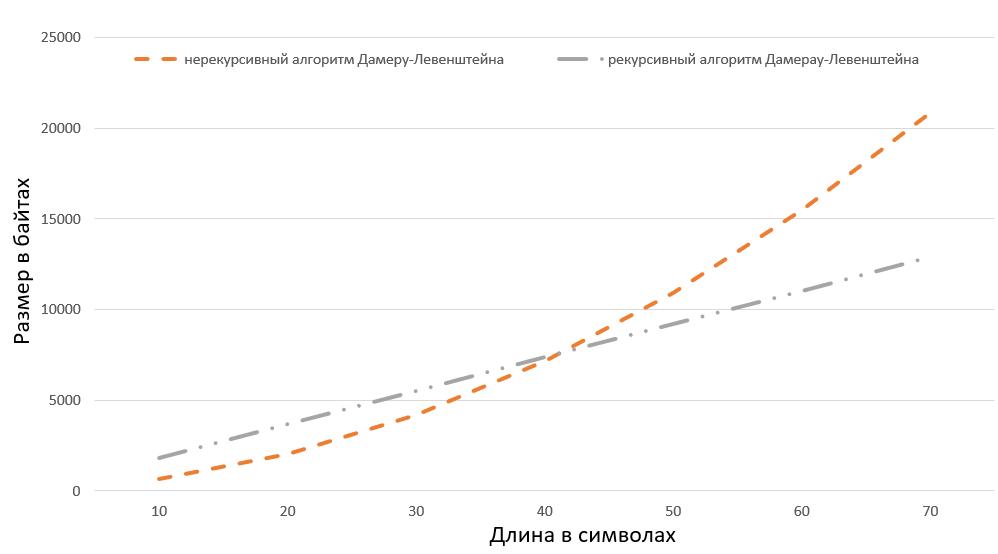
\includegraphics[height=0.3\textheight]{img/diag_04.png}
	\caption{Сравнение по памяти алгоритмов поиска расстояния Дамерау-Левенштейна --- итеративной и рекурсивной реализации}
	\label{plt:memory_1}
\end{figure}

\clearpage

\section{Вывод}

В данном разделе было произведено сравнение количества затраченного времени и памяти алгоритмов поиска расстояний Левенштейна и Дамерау-Левенштейна. Наименее затратным по времени оказался итеративный алгоритм нахождения расстояния Левенштейна.

Приведенные характеристики показывают, что рекурсивная реализация алгоритма в 21 раз проигрывает по времени. В связи с этим, рекурсивные алгоритмы следует использовать лишь для малых размерностей строк (1 -- 4 символа).

Так как во время печати очень часто возникают ошибки связанные с транспозицией букв \cite{ulianov}, алгоритм поиска расстояния Дамерау-Левенштейна является наиболее предпочтительным, не смотря на то, что он проигрывает по времени и памяти алгоритму Левенштейна.

Рекурсивная реализация алгоритма поиска расстояния Дамерау-Левенштейна будет более затратным по времени по сравнению с итеративной реализацией алгоритма поиска расстояния Дамерау-Левенштейна, но менее затратным по памяти по отношению к итеративному алгоритму Дамерау-Левенштейна.
